\usepackage{graphicx}
\section{Desarrollo del proyecto}
Se comenzó el proyecto buscando el robot adecuado para usar en el simulador Gazebo, se decidió utilizar este entorno de simulación porque es el que resultaba más familiar a los componentes del grupo.\\
Esta primera parte dió más problemas de los que se preveía. 
Inicialmente, se escogió el robot Pepper, pero este robot dió dos problemas importantes:
\begin{itemize}
Por un lado, cuando se iniciaba la simulación con las físicas activadas, el robot comenzaba a rotar sobre sí mismo, hasta que terminaba cayendo al suelo como se muestra en las siguientes imágenes, una de ellas al comienzo de la rotación, y la segunda con el robot ya en el suelo. Esto se consiguió arreglar actualizando la versión de gazebo, desde la versión 7.0 a la 8.0
\begin{figure}
  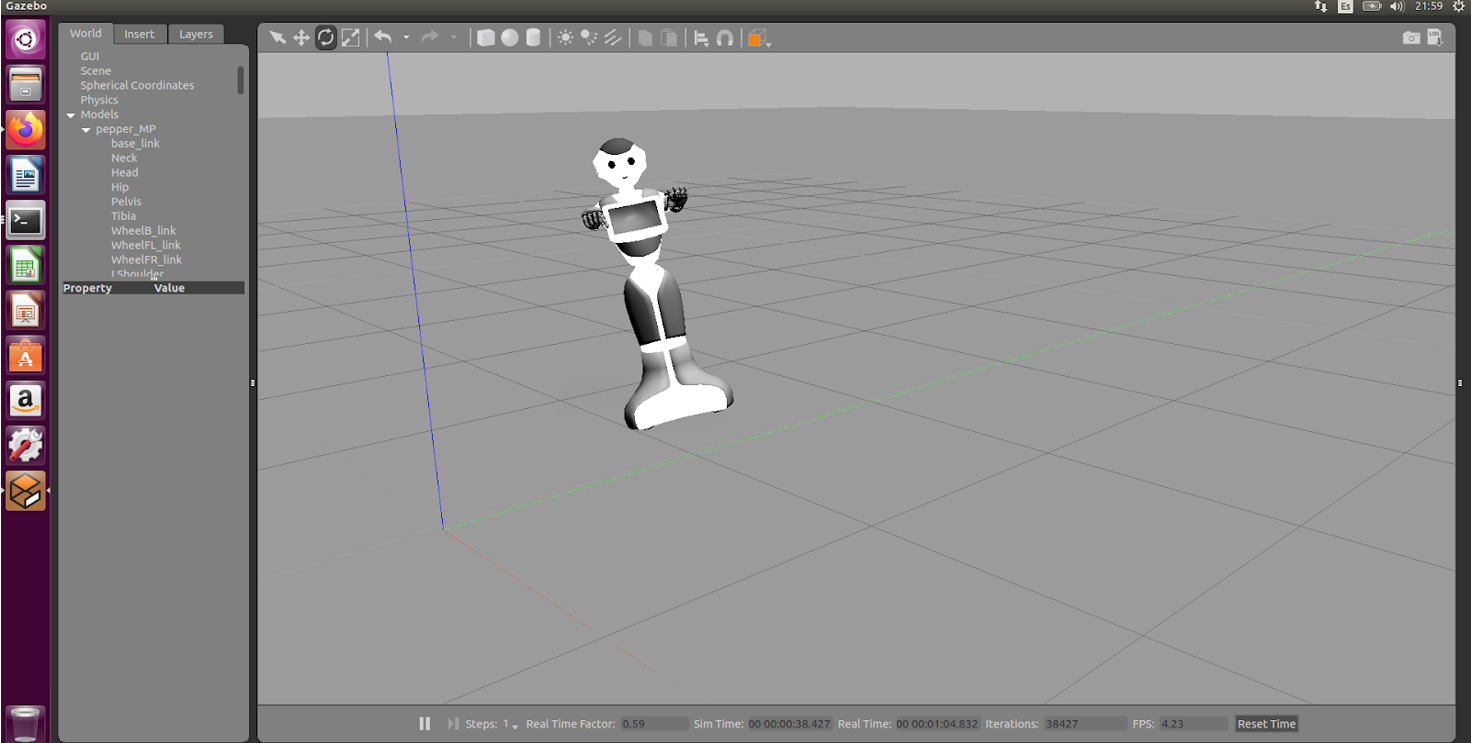
\includegraphics{texImages/peppergiro.png}
\end{figure}
\begin{figure}
  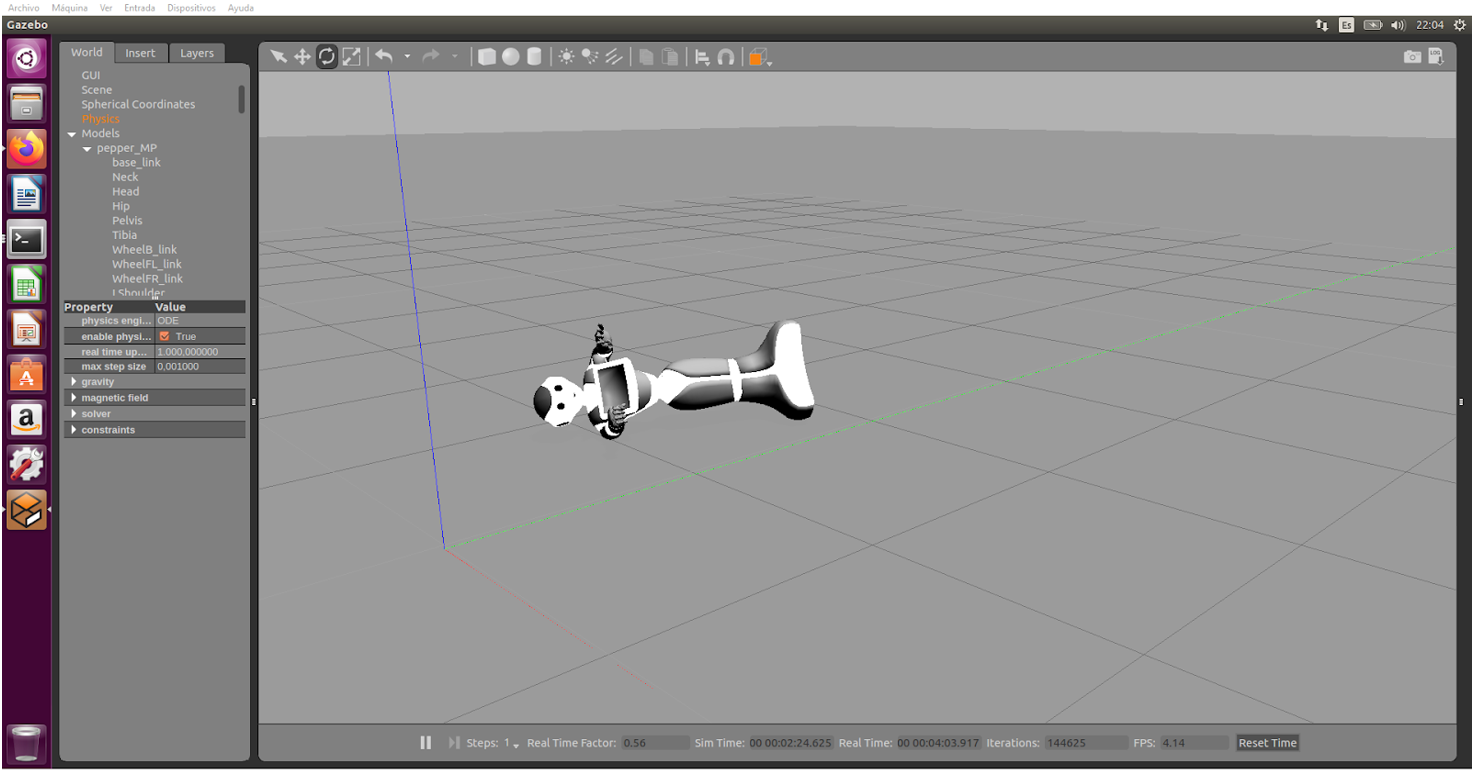
\includegraphics{texImages/peppersuelo.png}
\end{figure}
El segundo problema apareció con respecto a la mano izquierda del robot, una vez comenzaba la simulación las falanges de los dedos se comportaban defectuosamente, de tal modo que se acaban introduciendo dentro de la propia mano, esto se intentó arreglar modificando las inercias en el código URDF, pero no se consiguió alcanzar un comportamiento realista.\\
\end{itemize}
También se intentó cambiar esa mano por otra clase de efector final diferente que también nos pudiera servir para la tarea a realizar. Pero tampoco dió resultado, por lo que se optó por elegir otro modelo de robot diferente.\\
\begin{figure}
  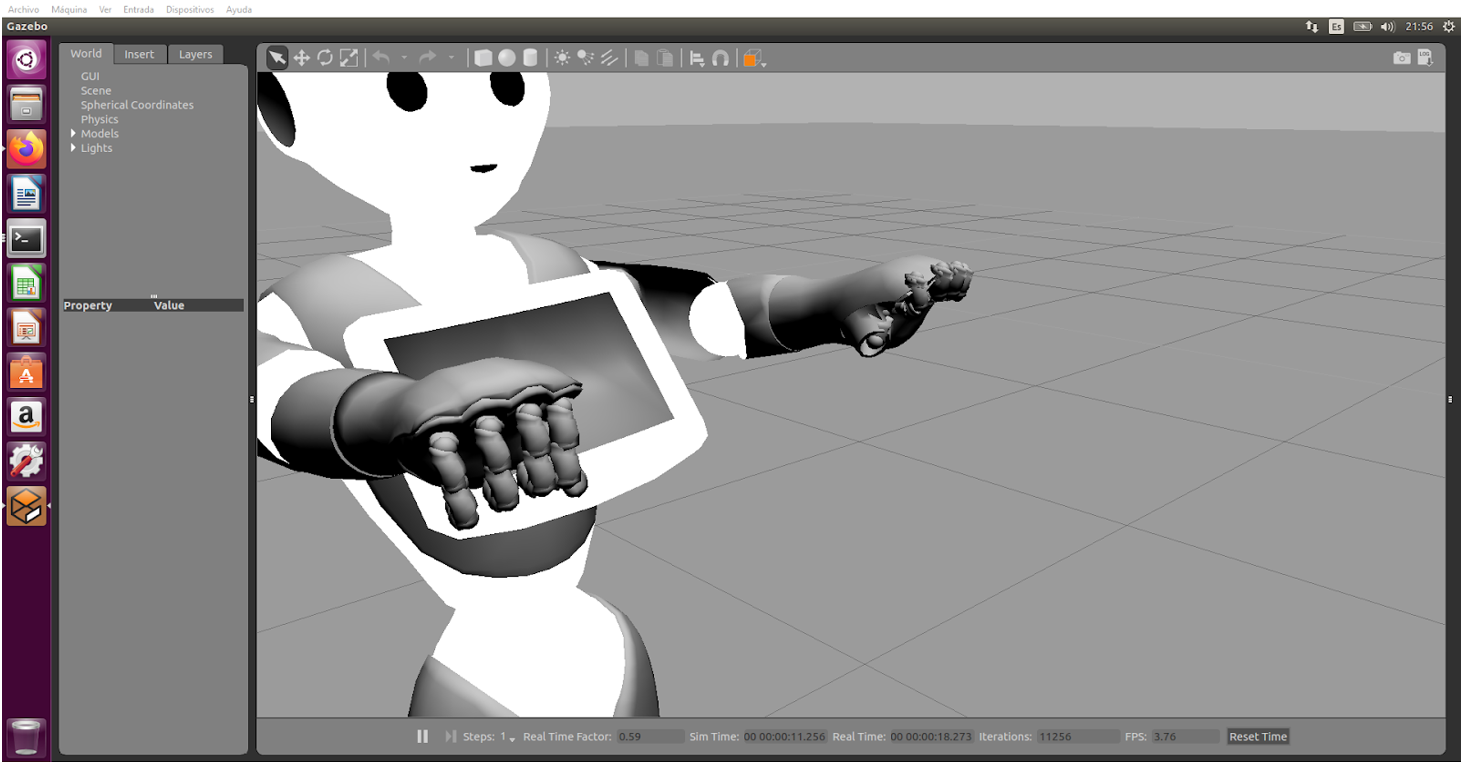
\includegraphics{texImages/peppermano.png}
\end{figure}
El catálogo de robots antropomórficos que encontramos disponibles para ROS Kinetic (la versión que disponíamos en la máquina virtual) no era muy extensa, pero finalmente conseguimos instalar el robot TiaGO, que sí que funcionaba correctamente sobre la versión de Gazebo 7.0.\\
\begin{figure}
  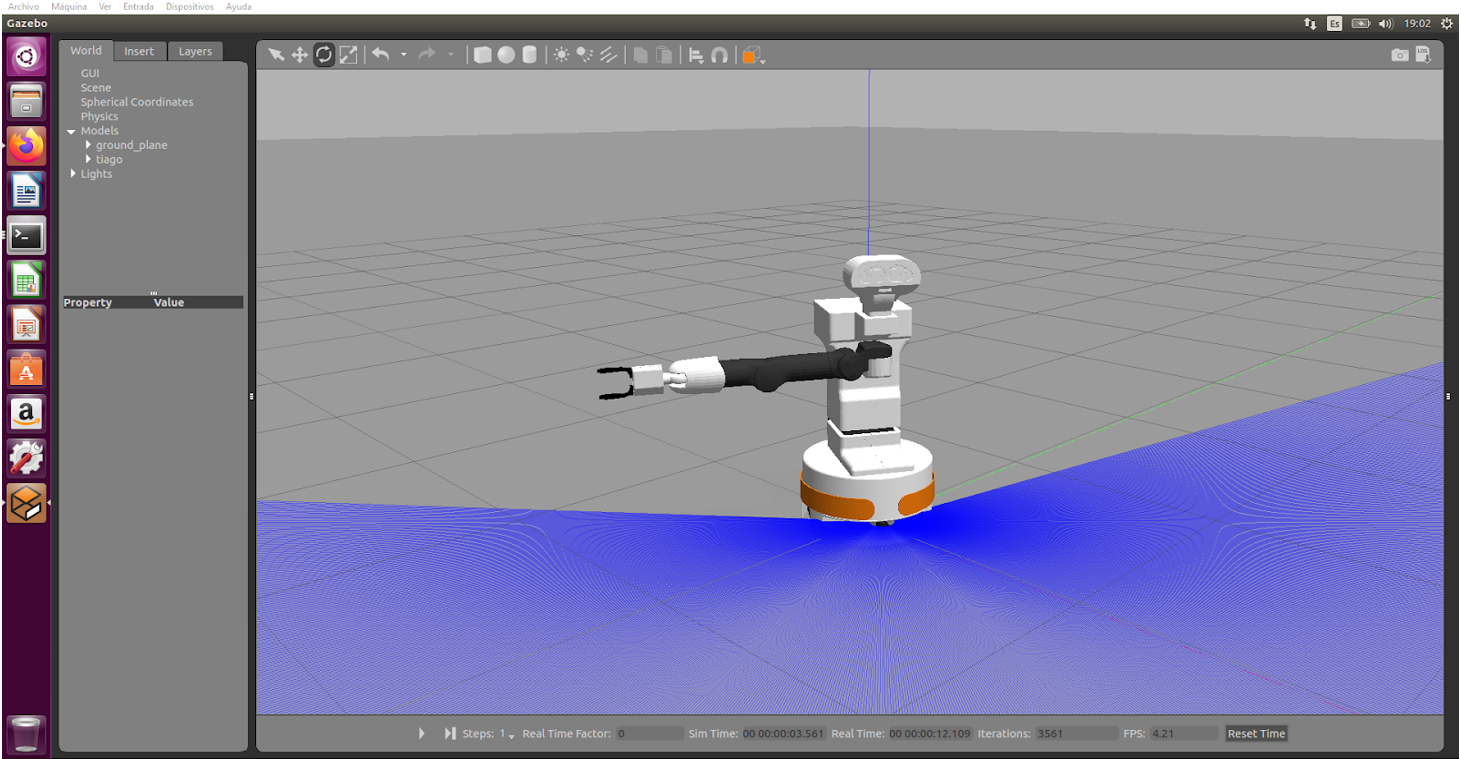
\includegraphics{texImages/tiago.png}
\end{figure}
Una vez seleccionado el robot adecuado se procede a la instalación de Openpose, que también da bastantes problemas para su correcta instalación, con lo cual el proyecto se retrasa todavía más.\\
Una vez correctamente instalado Openpose, este se utiliza en combinación con una cámara de profundidad Intel® RealSense™ D435, que nos permitirá obtener los valores de posición en 3D. El código que hemos necesitado implementar para conseguir esto se encuentra en el archivo adjunto openposeRealsense.py debidamente comentado.\\
